\subsection{Coordination and integration in Jazz}
The Jazz team is a large distributed team and uses the Jazz platform for
development. The Jazz development involves distributed collaboration over 16
different sites located in the United States, Canada, and Europe. Seven sites are
active in Jazz development and testing. There are 151 active contributors
working in 47 teams at these locations, where contributors belong to multiple
teams. Each team is responsible for developing a subsystem or component of Jazz.
The team size ranges from 1 to 20 and has an average of 5.7 members. The number
of developers per geographical site ranges from 7 to 24 and is 14.8 in average.

The project uses the \emph{Eclipse Way} development process~\cite{frost:ieeesoftware:2007}.
It defines six-week iteration cycles, which are separated into planning,
development and stabilization activities. A project management committee
formulates the goals and features for each release at the beginning of the each
iteration, and \et{Work Item}s represent assignable and traceable tasks for each
team.

\begin{figure}[t]
\begin{center}
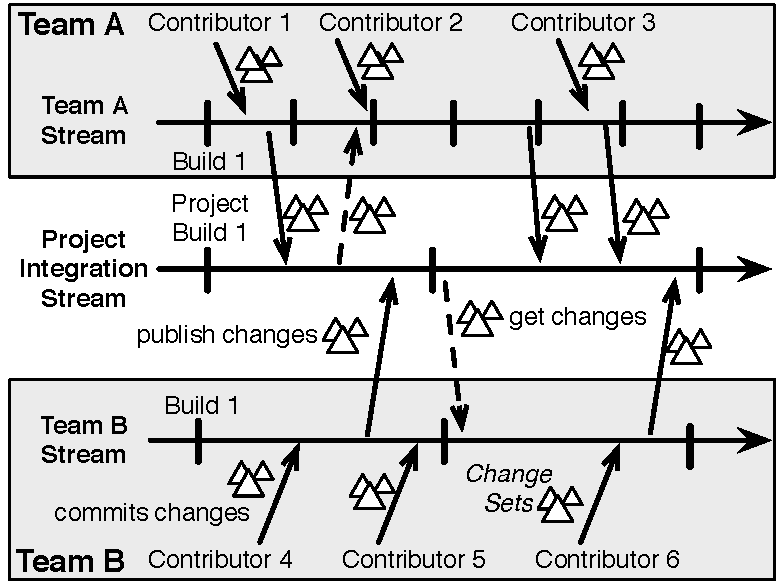
\includegraphics[width=8.3cm]{figures/BuildResult}
%\caption{Illustrates the exchange of change sets between different source code
%streams and the results of building the source code of the streams in time. Team
%members collaborate and interchange source code on a team related stream, while
%inter-team collaboration occurs on an integration stream.}
\caption{Teams contribute to their own source streams, which are then merged into one project stream.}
\label{fig:BuildResult}
\end{center}
\end{figure}


As illustrated in Figure~\ref{fig:BuildResult}, the coordination process within
each iteration requires the integration of subsystems developed by individual
Jazz teams in a major milestone build of the product (referred to as beta build).
Each team owns a source code \et{Stream} for collaboration and concurrent
implementation of the subsystem. A Stream is the Jazz equivalent to a branch of a
source configuration management system such as Subversion.

A continuous integration process takes place at team-level or project-level. In
frequent intervals, each integration build (referred to a build henceforth)
compiles, packages, and tests the source code of a stream. At the team-level,
contributors commit code changes that are encapsulated in \et{Change Sets} from
their own workspace to the \et{Team Stream}. The team integrations build the
subsystem developed by the team. Once a team has a stable version within the Team
Stream, the team publishes the change sets into the Jazz \et{Project Integration
Stream} (see Figure~\ref{fig:BuildResult}). At the project level, the automated
Jazz integration builds the subsystems of all teams. The Jazz project-level
integration takes place \et{nightly}, \et{weekly}, and at the end of each
iteration -- \et{beta} build.

\subsection{Coordination outcome measure}
In our study we conceptualize the coordination outcome by the \et{Build Result},
which is regarded as a coordination success indicator in Jazz and can be \error,
\texttt{WARNING} or \ok. We analyze build results to examine the integration
outcomes in relation to the communication necessary for the coordination of the
build.

Conceptually, the \texttt{WARNING} and \ok\ build results are treated similar by
the Jazz team, as they require no further attention or reaction from the
developers. In contrast, \error\ build results indicate serious problems such as
compile errors or test failures and require further coordination, communication
and development effort. We thus treated all \texttt{WARNING}s as \ok s to clearly
separate between failed and successful builds in our conceptualization of
coordination outcome.


\subsection{Communication in Jazz}

\et{Commenting} on work items is the main task-related communication and
collaboration channel used by Jazz. \et{Work Item}s represent single assignable
and traceable tasks. A set of work items defines the tasks for each team in each
iteration. Different types of work items represent defects, enhancements, and
general tasks. The work items are assigned to and owned by contributors. The
coordination necessary around the implementation of a work item is facilitated by
contributors commenting or observing the communication around work items.









%%%%%%%%%%%%%%%%%%%%%%%%%%%%%%%%%%












\subsection{Development and Builds in the Jazz Team}
%\subsection{Coordination and integration in Jazz}
The Jazz\tm\ team is a large distributed team and uses the Jazz\tm\ platform for
development. The Jazz\tm\ development involves distributed collaboration over 16
different sites located in the United States, Canada, and Europe. Seven sites are
active in Jazz development and testing. There are 151 active contributors
working in 47 teams at these locations, where developers can belong to multiple
teams. Each team is responsible for developing a subsystem or component of Jazz\tm\.
The team size ranges from 1 to 20 and has an average of 5.7 members. The number
of developers per geographical site ranges from 7 to 24 and is 14.8 in average.

The project uses the \emph{Eclipse Way} development process~\cite{frost:ieeesoftware:2007}.
It defines six-week iteration cycles, which are separated into planning,
development and stabilization activities. A project management committee
formulates the goals and features for each release at the beginning of the each
iteration, and \emph{work items} represent assignable and traceable tasks for each
team.
Furthermore, the Jazz\texttrademark\ team's development process demands that the developers coordinate using work item discussion. 

The coordination process within
each iteration requires the integration of subsystems developed by individual
Jazz\tm\ teams in a major milestone build of the product.
Each team owns a source code Stream for collaboration and concurrent
implementation of the subsystem. A Stream is the Jazz\tm\ equivalent to a branch of a
source configuration management system, such as Subversion.

A continuous integration process takes place at team-level or project-level. In
frequent intervals, each integration build (referred to a build henceforth)
compiles, packages, and tests the source code of a stream. At the team-level,
contributors commit code changes that are encapsulated in change sets from
their own workspace to the Team Stream. The team integrations build the
subsystem developed by the team. Once a team has a stable version within the Team
Stream, the team publishes the change sets into the Jazz\tm\ Project Integration
Stream. At the project level, the automated
Jazz\tm\ integration builds the subsystems of all teams. 
%The Jazz project-level
%integration takes place \et{nightly}, \et{weekly}, and at the end of each
%iteration -- \et{beta} build.

%%%%%%%%%%%


%We analyze builds created by IBM's Jazz\texttrademark\ development team.
%The Jazz team builds on a regular basis on a nightly and weekly basis.
%Those builds are both on a component and on a project basis.
%
%The Jazz team uses the software they develop the IBM Jazz\texttrademark.
%IBM Jazz\tm\ integrates both source code control and task management.
%Additionally you can also define build schedules as well as general development processes, such as SCRUM.
%
%Thus, the Jazz repository contains all the information from builds over source code changes to tasks, such as bug fixes.
%One advantage of working with he Jazz repository is that links between builds and changes, and changes and tasks are explicit.
%This means we know from the repository which changes contributed to a build and which changes where made to accomplish a task.
%Using this information we can infer which tasks influenced which builds.
%
%The Jazz development team follows the Eclipse Way of development~\cite{frost:ieeesoftware:2007}.
%The team was between April and July 2008 on a six week development cycle during which a set of features and bug fixes needs to be implemented.
%Instead of extending the cycles when features or bug fixes would take longer to complete they reschedule it for the next cycle.
%
%Another important aspect to their process directly impacts the way they communicate or record their communication.
%Since the Jazz development team is distributed across several sites in North America and Europe they implemented a process that enforces them to record all their communication around any task in the repository.
%This is a best practice implemented by the former Eclipse developer to ensure that people offside do know what's going on and to enable them to contribute.

% some stats about the repository and the team
We mined the Jazz project repository between April and July 2008, and analyzed a
total of 328 builds, out of which 99 were failed and 227 were successful.
Table~\ref{tab:jazzbuildinfo} contains summary statistics describing the Jazz\tm\
repository. We report different aggregations (minimum, average and maximum) of
number of work items, change sets, and developers over all builds. 






%%%%%%%%%%%%%%%%%%%%%%%%%%%%%%%%%%%%%%%




\subsection{IBM Rational Team Concert Case Study}

%In our research we conducted a study on RTC by IBM.
%We choose this project because it is a project with high coordination needs and a large amount of recorded communication.
IBM Rational Team Concert, or \textbf{RTC}, is a collaborative software development tool built on the Jazz\textsuperscript{\texttrademark} architecture. It incorporates the integrated development environment, the source-code control system, the issue-tracking system, and collaborative development tools. The RTC team self-hosts, meaning that the team uses its own software to develop subsequent versions.

The following qualities make RTC an attractive case in which to study
socio-technical coordination: (1) the distributed team, (2) the iterative
process, and (3) the rich data repository. Because distribution makes coordinating work difficult~\cite{hinds:cscw:2006,herbsleb2003:speed}, RTC is supposed to enhance communication among project members by providing collaborative facilities~\cite{frost:ieeesoftware:2007}. Developers explicitly record communication across sites using the product.
RTC's iterative process encourages developers to ``build early and often''. In addition to supporting continuous builds, RTC does frequent integration builds, providing a large amount of data to analyse.
% The encouraged community involvement and the openness to the community poses extra stress on the developers because of the increased information input they get~\cite{fussell98:overload}.

At the time of our study, the RTC development team involved a team distributed over 16
different sites located in the United States, Canada, and Europe. Seven sites were
active in RTC development and testing. There were 151 active contributors
at these locations. Each team, which was not necessarily confined to one geographical location,
was responsible for developing a component of RTC.
The team sizes ranged from 1 to 20 and had an average of 5.7 members. The number
of developers per geographical site ranged from 7 to 24 and was 14.8 on average.

The project uses the \emph{Eclipse Way} development process~\cite{frost:ieeesoftware:2007}.
It defines six-week iteration cycles, which are separated into planning,
development and stabilization activities. A project management committee
formulates the goals and features for each release at the beginning of the each
iteration, and \emph{work item}s represent assignable and traceable tasks for each
team. RTC's process encourages frequent building, including continuous, nightly, weekly, and integration builds.

%The RTC team is self-hosting, meaning that it uses the software system that it develops. Of particular note is the team's use of Rational Team Concert, which is a client-sidedevelopment environment that integrates programming, source code control, report generation and delivery, issue-tracking, and project planning into one system.

One unique aspect of RTC is its ``open-commercial'' development model. RTC is a commercial product developed by IBM, but has a publicly-accessible issue-tracking and reports system. This open-commercial model allows a large amount of information to flow into the team from the community.
Communication between individuals is done through the issue-tracking comments, through instant messaging, through Internet Relay Chat, by phone, and face-to-face. Personal email is discouraged. The team uses a mailing list to deliver announcements, such as server maintenance schedules. 
%The team recommends that discussions that do not occur in public channels are summarized as work item comments so that remote team members are able to track decisions and rationales.




%%%%%%%%%%%%%%%%%%%%%%%%%%%%%%%%%%%%%%%%%%%%%%%%%%%%%%%%



\subsection{Study Setting}
\label{sec:rtc}
 
%(MORE HERE FROM PREVIOUS DESCRIPTIONS OF JAZZ IN OUR PUBS) 
Rational Team Concert is a scalable and extensible team collaboration platform that integrates source code management, issue tracking, and planning tools. The RTC platform uses a client-server architecture, with the server acting as a central data repository.
The team also uses RTC to develop RTC, and in this way RTC is a self-hosting project.
This helps the RTC team become aware of issues with the product before customers.% ANYTHING WE CAN SAY ABOUT ITS CUSTOMER BASE? 
The project follows a large scale iterative development process that emphasizes transparency~\cite{frost:ieeesoftware:2007}.
It defines six-week iteration cycles, which are  separated into planning, development and stabilization activities. A project management committee formulates the goals and features for each release at the beginning of each iteration, and the output of this process is assigned to the teams in the form of work items. The work items and nearly all documentation are publicly available.  %(except for the code repository)

The RTC development team has over 100 developers distributed across multiple sites in North America, Europe and Asia.  The RTC development team is subdivided into several teams that manage a component each, such as the source code system or the web user interface. To communicate with each other, especially across different geographical locations, the developers extensively use RTC's own issue and task management system. A particular characteristic of the RTC development environment---and one that made this study of communication behaviour around changesets possible---are explicit traceable links between work tasks, associated changesets, and developers' online comments about these tasks and changesets\footnote{Changesets in RTC are created in a developer workspace; each changeset consists of several changes to code files.}.
